\chapter{Physical Setup}\label{ch:physsetup}
\section{Centrifugal Pumps}

A pump is device used to move liquid through a piping system and to 
raise the pressure of the liquid. We will focus on explaining 
and describing only centrifugal pumps,
since this is the type of pump present in our setup. 

\subsection{Principle}

In 1689, physicist Denis Papin invented the centrifugal pump. 
It is the most commonly used type of pump, due to its simple construction,
relative low cost, reliability and quiet operation.

The pump is built on a simple principle: Liquid is led to the impeller hub
and by means of the centrifugal force it is flung towards the periphery of 
the impeller. 

Figure \ref{fig:pump_sections} represents two cross sections of a centrifugal pump.
\begin{figure}[h]
    \centering
    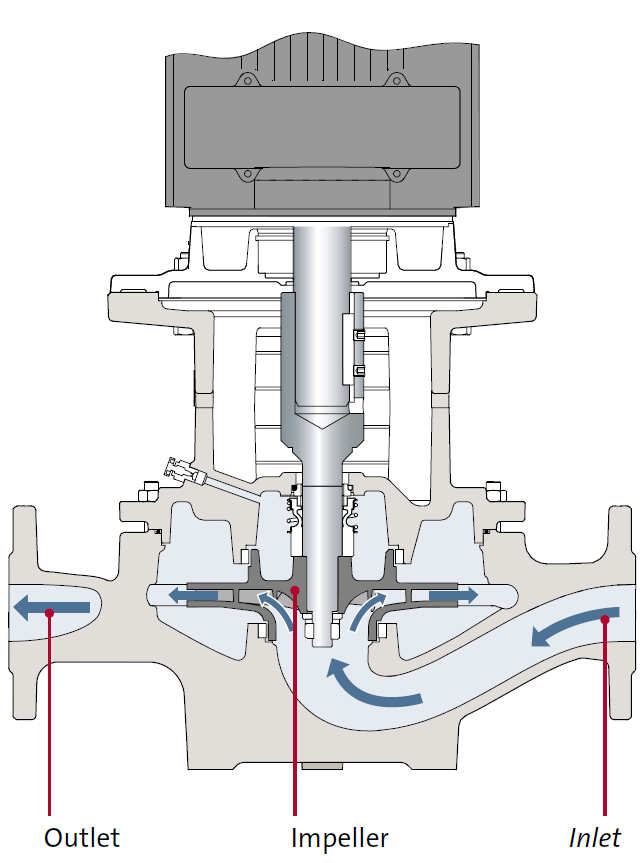
\includegraphics[width=0.3\linewidth]{figures/pump_cross_section.PNG}
    \qquad
    \hfill
    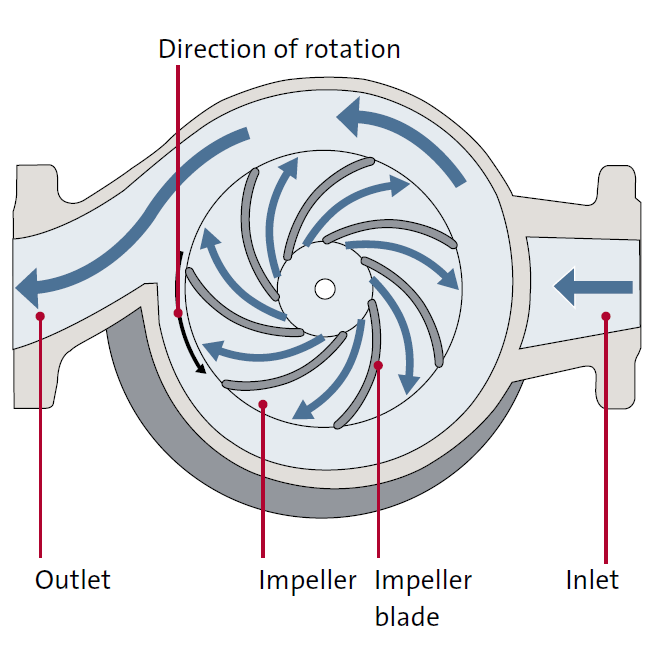
\includegraphics[width=0.3\linewidth]{figures/pump_above_view.PNG}
    \caption{Centrifugal Pump}
    \label{fig:pump_sections}
\end{figure}
\newpage

The fluid is sucked into the impeller at the impeller eye and flows through
the impeller channels formed by the blades between the shroud and hub.
The blades of the rotating impeller transfer energy to the fluid by
increasing velocity and pressure.

The design of the impeller depends on the requirements for application,
pressure and flow. The impeller is the primary component determining the pump performance. 
Pumps variants are often created only by modifying the impeller.

\subsection{Affinity Laws}
Affinity laws are mathematical relationships that provide a way to estimate the 
changes in performance of a pump, as a result of a change in one of the basic pump variables.
In it's simplest form, the term law, means a principle that has been proven true for all cases.

Equations for a specific centrifugal pump to determine flow, head and power curves 
for different motor speeds $N$ \cite{Volk2014}.
\begin{align*}
	\frac{Q_1}{Q_2} = \left(\frac{N_1}{N_2}\right)   &&
	\frac{H_1}{H_2} = \left(\frac{N_1}{N_2}\right)^2 &&
	\frac{P_1}{P_2} = \left(\frac{N_1}{N_2}\right)^3	
\end{align*} 

Equations for a specific centrifugal pump to determine flow, head and power curves 
for different impeller sizes $D$ \cite{Volk2014}.

\begin{align*}
	\frac{Q_1}{Q_2} = \left(\frac{D_1}{D_2}\right)   &&
	\frac{H_1}{H_2} = \left(\frac{D_1}{D_2}\right)^2 &&
	\frac{P_1}{P_2} = \left(\frac{D_1}{D_2}\right)^3
\end{align*} 

\newpage
\subsection{Performance Curves}
\subsubsection{Pump Head Curve}
A QH-curve or pump curve defines the head as a function of the flow. 
The flow is the rate of the fluid going through the pump. It is generally stated in
cubic meter per hour $[m^{3}/h]$. Figure \ref{fig:typicalPumpCurve} represents a typical

\begin{figure}[h]
	\centering
	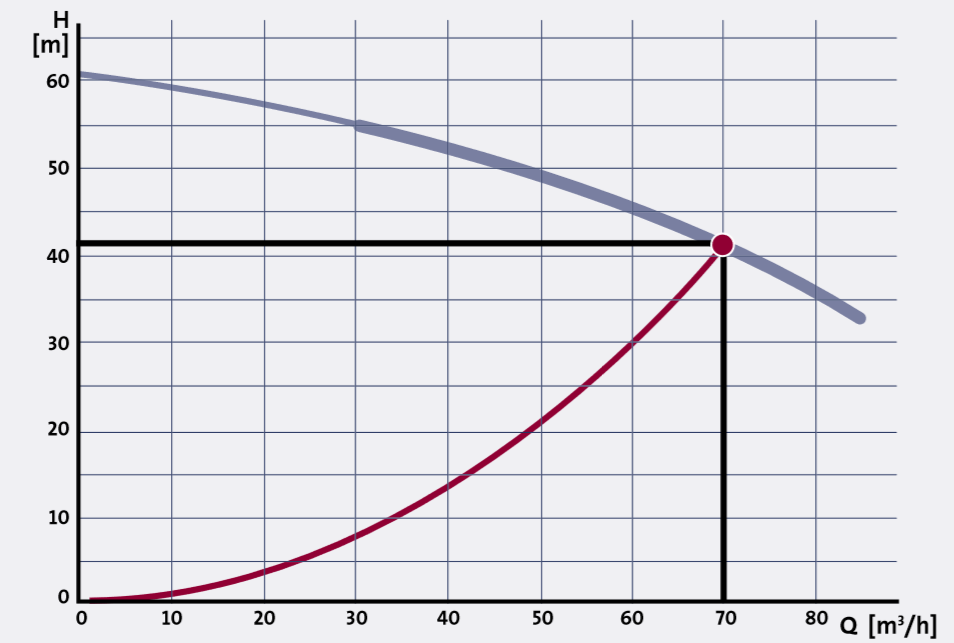
\includegraphics[width=0.8\textwidth]{figures/03physicalSetup/typicalHeadCurve.PNG}
	\caption{Typical Pump Head Curve}
	\label{fig:typicalPumpCurve}
\end{figure}

\subsubsection{Power Consumption Curve}
The relation between the flow and the power consumption can be seen in Figure \ref{fig:typicalPowerConsumptionCurve}.
Generally, the power consumption increases with the flow.

\begin{figure}[h]
	\centering
	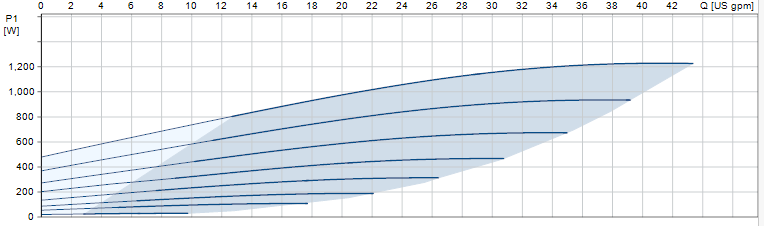
\includegraphics[width=0.9\textwidth]{figures/03physicalSetup/typicalPowerConsumptionCurve.PNG}
	\caption{Typical Power Consumption Curve}
	\label{fig:typicalPowerConsumptionCurve}
\end{figure}

\subsubsection{Efficiency Curve}
The efficiency of a pump, is the relation between the power delivered from the pump to the water,
and the power supplied to the shaft of the pump. Figure \ref{fig:typicalEfficiencyCurve} represents 
a efficiency curve of a pump.

\begin{figure}[h]
	\centering
	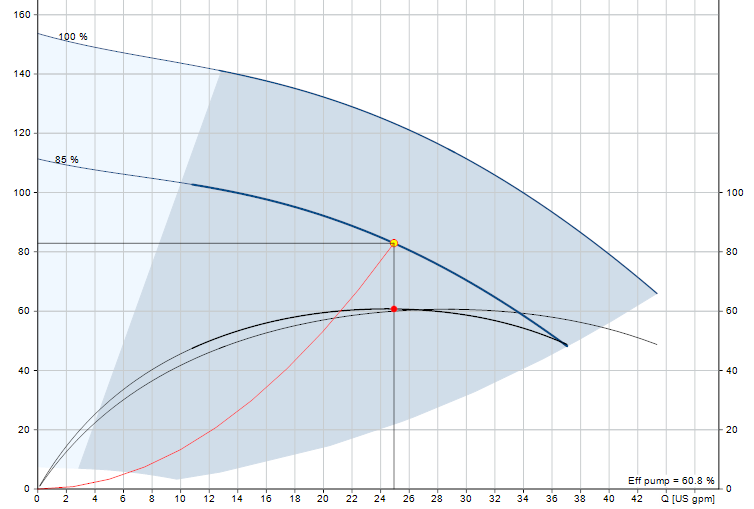
\includegraphics[width=0.9\textwidth]{figures/03physicalSetup/typicalEfficiencyCurve.PNG}
	\caption{Typical Efficiency Curve}
	\label{fig:typicalEfficiencyCurve}
\end{figure}

\subsubsection{NPSH - Curve (Net Positive Suction Head)}
The NPSH is the minimum required pressure that has to be present at the inlet to avoid cavitation.
The NPSH increases with the flow. Figure \ref{fig:typicalNPSHCurve} represents an NPSH - Curve
of a pump.

\begin{figure}[h]
	\centering
	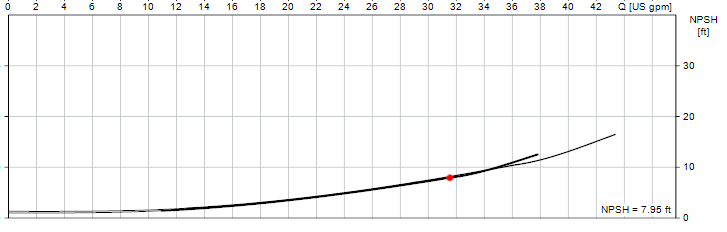
\includegraphics[width=0.9\textwidth]{figures/03physicalSetup/typicalNPSHCurve.PNG}
	\caption{Typical NPSH Curve}
	\label{fig:typicalNPSHCurve}
\end{figure}

\section{Pipes}
Pipes are a way of transporting liquids or gasses, inside a controllable environment.
They are used to interconnect the pumps and the tank and other peripherals.
One common analogy compares them to wires in electrical circuits.

Based on their diameters, material and shape,
they introduce resistance to the flow of the pumped medium.
Staying with the analogy to electrical circuits,
this can be compared to the cross sectional area and the specific resistance of a wire material.

\section{Valves}
A valve is a device used to regulate the flow of a gas or liquid through a piping system.
The valve built into our system is not used for regulatory purposes,
but only to simulate disturbances in the system.
Valves can be actuated by different means, such as air pressure, electric motors or rotary handles.

\section{Sensors}
Sensors were present on the setup. They were used to gather the data used throughout the report 
and closely monitor the system. The data gathered was used to determine various pump curves.

\subsubsection{Flow Meter}
After each pump, a magnetic flow meter is installed to measure the flow, and configured to measure 
cubic meters per hour.
\subsubsection{$\Delta$Pressure Sensor}
Pressure sensors are installed across the pump, measuring the pressure difference between two points.
One located before and the other located after the pump. They are configured tho measure in bars.
\subsubsection{Power Sensor}
A power sensor was used to closely monitor the power delivered to the pumps. The power was expressed
in Watts.
